% A LaTeX (non-official) template for ISAE projects reports
% Copyright (C) 2014 Damien Roque
% Version: 0.2
% Author: Damien Roque <damien.roque_AT_isae.fr>

\documentclass[a4paper,12pt]{book}
\usepackage[utf8]{inputenc}
\usepackage[T1]{fontenc}
%\usepackage[frenchb]{babel} % If you write in French
\usepackage[frenchb]{babel} % If you write in English
\usepackage{a4wide}
\usepackage{graphicx}
\usepackage{subfig}
\usepackage{tikz}
\usetikzlibrary{shapes,arrows}
\usepackage{pgfplots}
\pgfplotsset{compat=newest}
\pgfplotsset{plot coordinates/math parser=false}
\newlength\figureheight
\newlength\figurewidth
\pgfkeys{/pgf/number format/.cd,
	set decimal separator={,\!},
	1000 sep={\,},
}
\usepackage{grffile}

\usepackage{caption}

\usepackage{ifthen}
\usepackage{ifpdf}
\ifpdf
\usepackage[pdftex]{hyperref}
\else
\usepackage{hyperref}
\fi
\usepackage{color}
\hypersetup{%
	colorlinks=true,
	linkcolor=black,
	citecolor=black,
	urlcolor=black}

\renewcommand{\baselinestretch}{1.05}
\usepackage{fancyhdr}
\pagestyle{fancy}
\fancyfoot{}
\fancyhead[LE,RO]{\bfseries\thepage}
\fancyhead[RE]{\bfseries\nouppercase{\leftmark}}
\fancyhead[LO]{\bfseries\nouppercase{\rightmark}}
\setlength{\headheight}{15pt}

\let\headruleORIG\headrule
\renewcommand{\headrule}{\color{black} \headruleORIG}
\renewcommand{\headrulewidth}{1.0pt}
\usepackage{colortbl}
\arrayrulecolor{black}

\fancypagestyle{plain}{
  \fancyhead{}
  \fancyfoot[C]{\thepage}
  \renewcommand{\headrulewidth}{0pt}
}

\makeatletter
\def\@textbottom{\vskip \z@ \@plus 1pt}
\let\@texttop\relax
\makeatother

\makeatletter
\def\cleardoublepage{\clearpage\if@twoside \ifodd\c@page\else%
  \hbox{}%
  \thispagestyle{empty}%
  \newpage%
  \if@twocolumn\hbox{}\newpage\fi\fi\fi}
\makeatother

\usepackage{amsthm}
\usepackage{amssymb,amsmath}
\usepackage{array}
\usepackage{bm}
\usepackage{multirow}
\usepackage[footnote]{acronym}
\usepackage{multicol}

\newcommand*{\SET}[1]  {\ensuremath{\mathbb{#1}}}
\newcommand*{\VEC}[1]  {\ensuremath{\boldsymbol{#1}}}
\newcommand*{\FAM}[1]  {\ensuremath{\boldsymbol{#1}}}
\newcommand*{\MAT}[1]  {\ensuremath{\boldsymbol{#1}}}
\newcommand*{\OP}[1]  {\ensuremath{\mathrm{#1}}}
\newcommand*{\NORM}[1]  {\ensuremath{\left\|#1\right\|}}
\newcommand*{\DPR}[2]  {\ensuremath{\left \langle #1,#2 \right \rangle}}
\newcommand*{\calbf}[1]  {\ensuremath{\boldsymbol{\mathcal{#1}}}}
\newcommand*{\shift}[1]  {\ensuremath{\boldsymbol{#1}}}

\newcommand*{\eme}[1] {$#1^{\mbox{\footnotesize{ème}}}$}

\newcommand{\eqdef}{\stackrel{\mathrm{def}}{=}}
\newcommand{\argmax}{\operatornamewithlimits{argmax}}
\newcommand{\argmin}{\operatornamewithlimits{argmin}}
\newcommand{\ud}{\, \mathrm{d}}
\newcommand{\vect}{\text{Vect}}
\newcommand{\sinc}{\ensuremath{\mathrm{sinc}}}
\newcommand{\esp}{\ensuremath{\mathbb{E}}}
\newcommand{\hilbert}{\ensuremath{\mathcal{H}}}
\newcommand{\fourier}{\ensuremath{\mathcal{F}}}
\newcommand{\sgn}{\text{sgn}}
\newcommand{\intTT}{\int_{-T}^{T}}
\newcommand{\intT}{\int_{-\frac{T}{2}}^{\frac{T}{2}}}
\newcommand{\intinf}{\int_{-\infty}^{+\infty}}
\newcommand{\Sh}{\ensuremath{\boldsymbol{S}}}
\newcommand{\C}{\SET{C}}
\newcommand{\R}{\SET{R}}
\newcommand{\Z}{\SET{Z}}
\newcommand{\N}{\SET{N}}
\newcommand{\K}{\SET{K}}
\newcommand{\reel}{\mathcal{R}}
\newcommand{\imag}{\mathcal{I}}
\newcommand{\cmnr}{c_{m,n}^\reel}
\newcommand{\cmni}{c_{m,n}^\imag}
\newcommand{\cnr}{c_{n}^\reel}
\newcommand{\cni}{c_{n}^\imag}
\newcommand{\tproto}{g}
\newcommand{\rproto}{\check{g}}
\newcommand{\LR}{\mathcal{L}_2(\SET{R})}
\newcommand{\LZ}{\ell_2(\SET{Z})}
\newcommand{\LZI}[1]{\ell_2(\SET{#1})}
\newcommand{\LZZ}{\ell_2(\SET{Z}^2)}
\newcommand{\diag}{\operatorname{diag}}
\newcommand{\noise}{z}
\newcommand{\Noise}{Z}
\newcommand{\filtnoise}{\zeta}
\newcommand{\tp}{g}
\newcommand{\rp}{\check{g}}
\newcommand{\TP}{G}
\newcommand{\RP}{\check{G}}
\newcommand{\dmin}{d_{\mathrm{min}}}
\newcommand{\Dmin}{D_{\mathrm{min}}}
\newcommand{\Image}{\ensuremath{\text{Im}}}
\newcommand{\Span}{\ensuremath{\text{Span}}}


\newtheoremstyle{break}
  {11pt}{11pt}%
  {\itshape}{}%
  {\bfseries}{}%
  {\newline}{}%
\theoremstyle{break}

%\theoremstyle{definition}
\newtheorem{definition}{Définition}[chapter]

%\theoremstyle{definition}
\newtheorem{theoreme}{Théorème}[chapter]
\newtheorem{lemme}{Lemme}[chapter]
\newtheorem{corollaire}{Corollaire}[chapter]
%\theoremstyle{remark}
\newtheorem{remarque}{Remarque}[chapter]
\newtheorem{remarques}{Remarques}[chapter]
%\theoremstyle{plain}
\newtheorem{propriete}{Propriétée}[chapter]
\newtheorem{exemple}{Exemple}[chapter]

\parskip=5pt
%\sloppy

\usepackage{pdfpages}

\usepackage{chngcntr}
\counterwithout{figure}{chapter}
\counterwithout{table}{chapter}
\counterwithout{theoreme}{chapter}
\counterwithout{remarques}{chapter}
\counterwithout{definition}{chapter}
\counterwithout{lemme}{chapter}
\counterwithout{corollaire}{chapter}

\usepackage{longtable}
\usepackage{wrapfig}

\usepackage{hyperref}

\usepackage[margin=1in]{geometry}                
\geometry{letterpaper}                  
\usepackage{graphicx}
\usepackage{epstopdf}
\usepackage{hyperref}
\DeclareGraphicsRule{.tif}{png}{.png}{`convert #1 `dirname #1`/`basename #1 .tif`.png}
\usepackage{cite}

\usepackage[utf8]{inputenc}
\usepackage[T1]{fontenc}

\usepackage{amsmath}

\DeclareMathOperator{\EX}{\mathbb{E}}



\usepackage{amssymb}

\begin{document}

%%%%%%%%%%%%%%%%%%
%%% First page %%%
%%%%%%%%%%%%%%%%%%

\begin{titlepage}
\begin{center}
	

{\large RESYS Project}\\[0.5cm]

% Title
\rule{\linewidth}{0.5mm} \\[0.4cm]
{ \huge \bfseries Differentiation of hematopoietic precursors in embryos\\[0.4cm] }
\rule{\linewidth}{0.5mm} \\[1.5cm]

\vspace{2cm}

% Author and supervisor
\noindent
\begin{minipage}{0.4\textwidth}
  \begin{flushleft} \large
    M.~Jeremie \textsc{Perrin} \\ \small \textit{M2 BIM student}\\ \small \textit{ENS Cachan}\\
  \end{flushleft}
\end{minipage}%
\begin{minipage}{0.4\textwidth}
  \begin{flushright} \large
    M.~Corbin \textsc{Hopper} \\ \small \textit{M2 MPRI student}\\
  \end{flushright}
\end{minipage}

\vfill

% Bottom of the page
{\large  2019 -- 2020}

\end{center}
\end{titlepage}

\section*{The Dataset}
\subsection*{The Early Hematopoietic process}
	The biological process we are studying is one of differentiation of multipotent precursor cells \textit{Hemangioblasts} into hematopoietic and endothelial cells alike. In the mouse embryo, there is emergence of blood cells at day 7 in the yolk sac and this is the marker of the beginning of the hematopoiesis. Both the Hematopoietic Stem Cells (HSC) and the Endothelial Stem Cells (EPC) originate from these multipotent precursor cells. The blood cells will be formed by differentiation of the HSCs while the vasculature (tissue of the blood vessels) will be formed through differentiation of the ESCs.

\subsection*{The Experiment}
	In the paper \textit{Decoding the Regulatory Network for Blood Development from Single-Cell Gene Expression Measurements}, single-cell gene expression data was used in order to infer the regulatory networks at work during the hematopoietic differentiation process. It is known that blood development
	initiates at gastrulation from mesodermal cells, which initially have the potential to form blood, endothelium and smooth muscle cells. They showed that single-cell analysis of a developing organ coupled with computational approaches can reveal the transcriptional programs that control organogenesis.\\
	In order to acquire the data necessary they sampled single-cells in \textit{in vivo} mice embryos. The cells were sampled from the mesoderm and their potential to differentiate into blood cells was asserted thanks to expression of Flk1 and Runx1 expression. The sampling was done at four distinct time points.\\
	Those four times points define groups of cells, which are not hemogeneous since the differentiation process is asynchronous. That is to say some cells begin their differentiation process earlier than others :
	\begin{itemize}
		\item[E7.00] At this time point the cells are labeled "PS"
		\item[E7.50] –––––––––––––––––––––––––––––––––– "NP"
		\item[E7.75] –––––––––––––––––––––––––––––––––– "HF"
		\item[E8.25] At this time points cells were categorized into two different set. Those cells which expressed \textit{GFP} were labeled "4SG" and where considered as putative blood cells while those that did not where labeled "4SFG" and considered as putative endothelial cells. 
	\end{itemize}
	At each time points gene expression of a set of genes was measured in each cell, these genes were selected by hand as they were known to play a role in the process. Forty-six genes were selected, out of those : four were housekeeping genes in order to assess the quelity of the measures. Nine were markers known to identify the different cell states and thirty-three were transcription known to play a role in the transcriptional program underlying the differentiation process. 
\subsection*{Categorizing Genes}
	 To be pertinent in our analysis we first need to categorize the genes into the different cell states they belong to. We use the literature to guide us in our task. In the article, the authors underlign groups of genes as being caracteristic of the two end states:
	\begin{itemize}
		\item[$\bullet$] For Hematopoietic Cells : Hbb-bH1, Gata1, Nfe2, Gfi1b, Ikzf1 (Ikaros) and Myb
		\item[$\bullet$] For Endothelial Cells : Erg, Sox7, Sox17, Hoxb4, Cdh5
	\end{itemize}
	\paragraph{}
	In order to build our own gene categories, we have proceeded in the following way. Each gene is represented by 5 values, those are the mean expression at each sampling points. Before doing unsupervised clustering we wanted to see if the genes were spatially grouping in terms of when they were expressed and how much they were expressed. We therefore ran a Principal Component Analysis (see Fig.~\ref{fig:genePCA}).Using this two dimensional representation of the data we were able to see that the genes characteristic of the different end stages grouped together. We separated the data into three clusters using K-Means algorithm (see again Fig.~\ref{fig:genePCA}).
	
	\begin{figure}[h!]
		\centering
		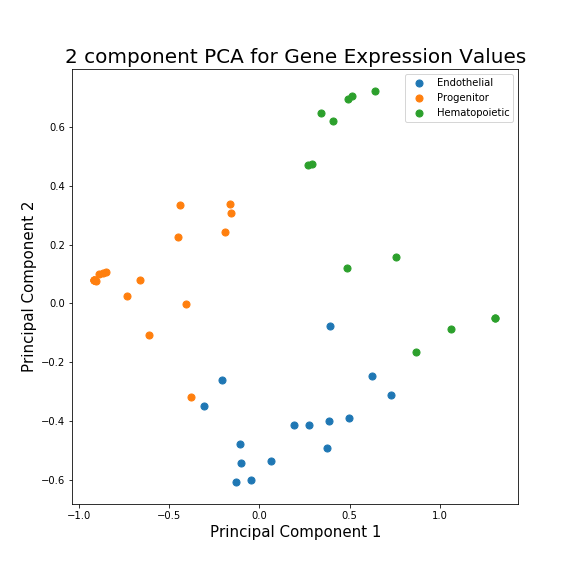
\includegraphics[height = 0.4\textheight]{../Preliminary/genepca.png}
		\caption{Genes represented after PCA transformation and grouped by unsupervised clustering into three clusters.}
		\label{fig:genePCA}
	\end{figure}
		We then plotted the actual mean expression values of the different genes grouped by their infered categories (see Fig.~\ref{fig:meangene}). We clearly see the distinction in between groups, the clear expression of genes categorized as Hematopoietic in the 4SG stage as well as the expression of Endothelial genes in the 4SFG stage. 
	\begin{figure}[h!]
		\centering
		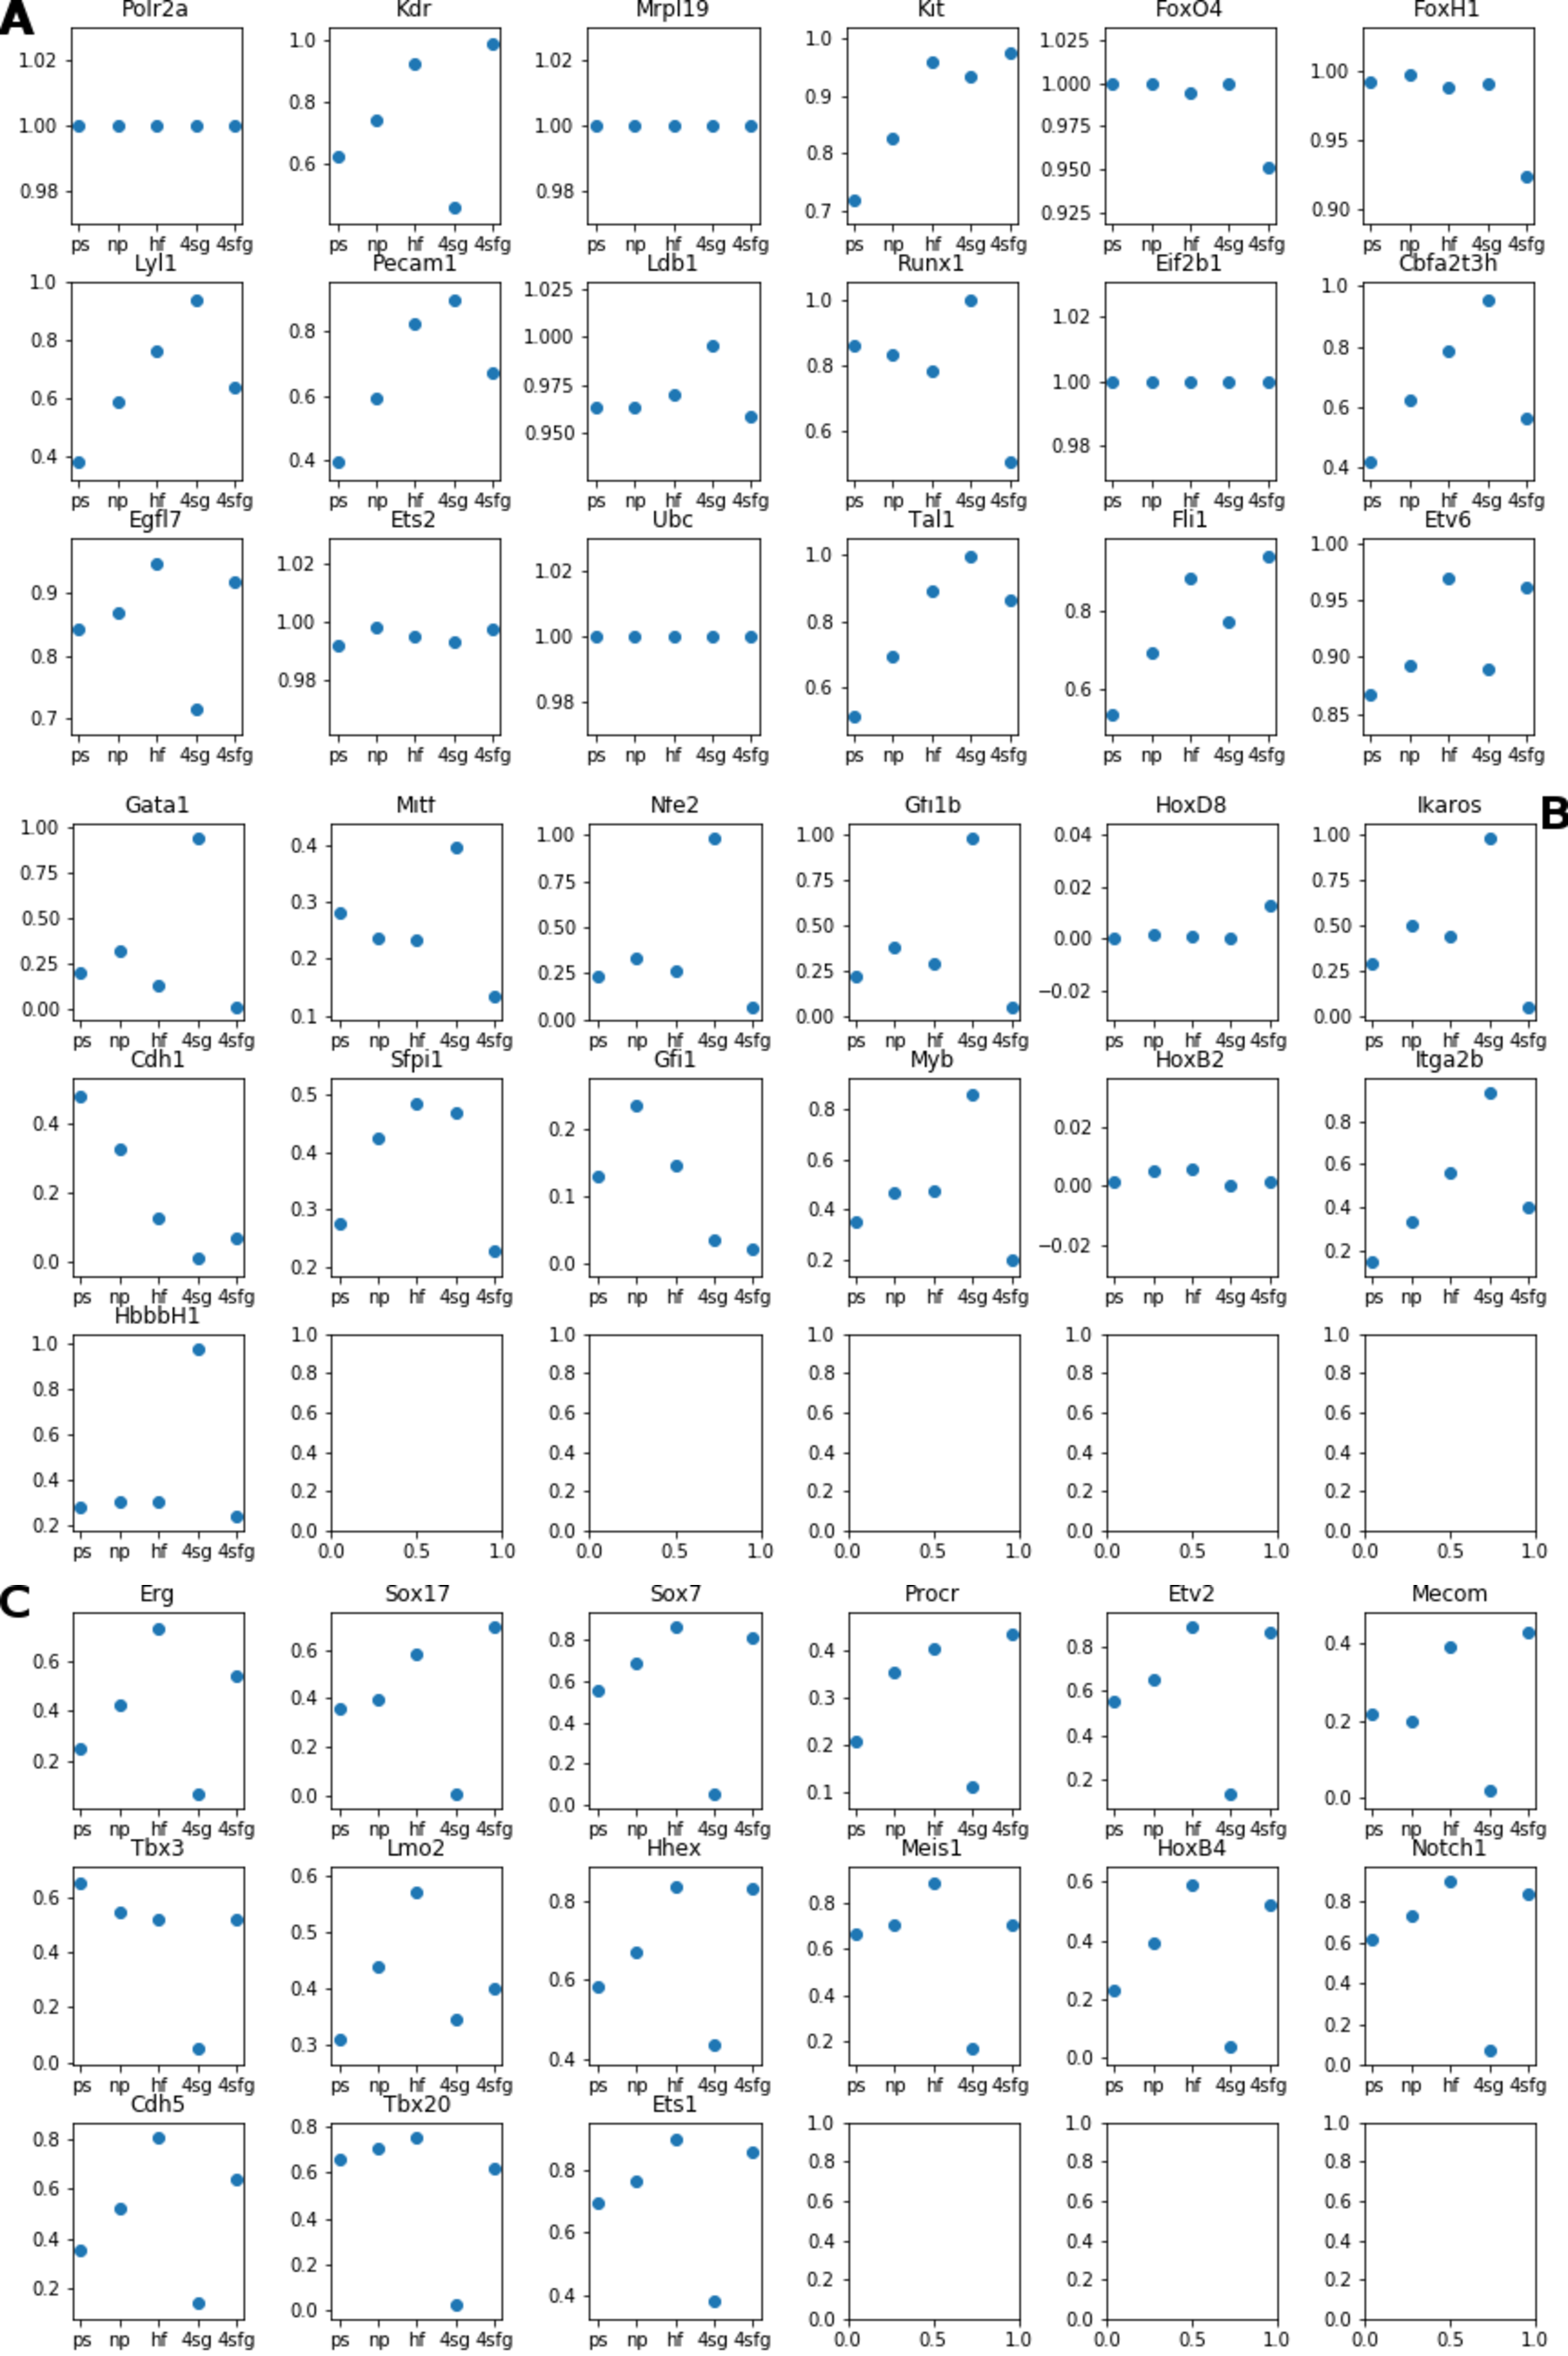
\includegraphics[width = 0.9\linewidth, height = 0.8\textheight]{../Preliminary/exptot.pdf}
		\caption{Mean gene expression values throughout the experiment. \textbf{A} Precursor genes \textbf{B} Hematopoietic genes \textbf{C} Endothelial genes}
		\label{fig:meangene}
	\end{figure}

\clearpage
 \section*{Conditional Entropy Based Network Inference}
 %need better notation for in edges in v, number eqns properly, make notation more consistent
 % shrink some equations
 % why x -> y -> z
 % poss check for which genes changeH=0 and strongly argue for ignoring them
 % more explanation as to why and issue with finite m?
 % more bio angle, esp at start
 
 \subsection*{Approach}
 
 One approach attempts to use conditional entropy to infer a directed graph. Although it is ultimately not robust on real data sets, it is used as a preprocessing step in the final network inference. Given that the hemapoeitic data lacks a clear temporal structure, inference about paths seem dubious. Instead, this approach considers each gene independently and appraises the most likely set of genes that regulate it. The goal is to minimize the conditional entropy of each vertex, given its input edges, relative to that of a random process. A predecessor is a vertex with a directed edge to its successor. However, the edges remain unsigned, the transfer function unspecified, and latent variables are not inferred.
 
 Conditional entropy of a vertex given its predecessors corresponds to the amount of randomness in the vertex that is unexplained by its predecessors. The set of genes that regulates another gene should minimize the uncertainty about that gene relative to a random set of the same size. Given that biological processes are inherently stochastic, the approach should prevent certain spurious correlations. Say a network is organized such that $x \rightarrow y \rightarrow z$. Then $x$ should not form an edge to $z$, since $y$ would provide more certain information about $z$.
 
 Given a graph $G$ with vertices and edges $(V,E)$.  The goal is formally defined as follows:
 \begin{equation} \label{eq:1}
 \argmax_{E \in G} \sum_{v \in V} I(v;e_{in}) - \EX[I(A;B)]
 \end{equation}
 Where I(Y;X) is the mutual information between the random variables Y and X. $\EX[I(A;B)]$ refers to the expected mutual information of a subset of instances $A,B$ that are the same size as $v,e_{in}$,but drawn from random distributions. Over many random distributions, some small amount of distributions are expected to be correlated by chance. Equation \ref{eq:1} is then simplified as follows:
 $$\sum_{v \in V} \argmax_{e_{in} \in E} I(v;e_{in}) - \EX[I(A;B)] = \sum_{v \in V} \argmax_{e_{in} \in E} (H(v) - H(v|e_{in})) - \EX[H(A)-H(A|B)] 
 $$
 $$
 = \sum_{v \in V} \argmin_{e_{in} \in E} (- H(v) + H(v|e_{in})) - \EX[- H(A) + H(A|B)]
 $$
 Where I(Y;X) is the mutual information between the random variables Y and X. The entropy of $v$, $H(v)$, does not change over its set of input edges (and same for $H(A)$). Then equation \ref{eq:1} can be further rewritten as:
 \begin{equation} \label{eq:2}
 \sum_{v \in V} \argmin_{e_{in} \in v} H(v|e_{in}) - \EX[H(A|B)]  = \sum_{v \in V} \argmin_{e_{in} \in v} -\EX[H(A|B)]\sum_{(i,j) \in (v,e_{in})} - p(i,j)\log_2{p(i|j)}
 \end{equation} 
 Where H(Y|X) is the conditional entropy of the random variable Y, given X, and p(x,y) is the joint probability of events x and y occurring. One can sum over instances (say rows of a matrix) $(v,e_{in})_0 ...(v,e_{in})_n$, instead of summing over outcomes $(i,j) \in (v,e_{in})$:
 $$ \argmin_{e_{in} \in v} -\EX[H(A|B)] \sum_{k=0}^n - \log{p(v_k|e_{in_k})} = \argmax_{e_{in} \in v} -\EX[H(A|B)] \prod_{k=0}^n {p(v_k|e_{in_k})} $$
 It then becomes clear that the approach maximizes the log-likelihood of the probability of observing the activity of vertices given their immediate predecessors.
 
 It remains for $\EX[H(A|B)]$ to be simplified. Let $A$ be a vector of length $n$ and $B$ a matrix of dimensions $n$ by $m$. This corresponds to the case where the output of one vertex is being evaluated, relative to that of a subset of its predecessors.
 If $A,B$ are the same type of distribution, then:
 $$ \EX[H(A|B_m)] = \EX[H(A,B_m)-H(B_m)] = \EX[H(b_1,...,b_m, b_{m+1}) - H(b_1,...,b_m)] $$
 If there is enough data $\EX[H(b_m)]$ should approach the entropy of $n$ random vectors. In other words, as $n$ approaches infinity, the probability that all $m$ vectors are different approaches $1$, and so:
 $$ \EX[H(A|B)] \approx \log2(m+1) - \log2(m) $$
 Let $m = |e_{in}|$. Then equation \ref{eq:2} can be rewritten as:
 \begin{equation} \label{eq:3}
 \sum_{v \in V} \argmin_{e_{in} \in v} H(v|e_{in}) - \log_2(\frac{m+1}{m})
 \end{equation}
 
 \subsection*{Algorithm}
 An algorithm is designed for equation \ref{eq:3} and summarized in \ref{pseudocode}. The maximum likelihood approach has already been aggressively simplified by only considering the immediate neighbors of each node. An efficient algorithm should still avoid iterating over all possible edge combinations for each node. Since $H(Y|x_1,...,x_m) \leq H(Y|x_1,...,x_{m-1})$, one can safely start with all edges and iteratively remove them if:
 \begin{equation} \label{eq:4}
 \begin{split}
 H(Y|x_1,...,x_{m-1}) -  H(Y|x_1,...,x_m) \leq \EX[{H(a|b_1,...,b_{m-1}) -  H(a|b_1,...,b_m)}]  \\ \\
 H(Y|x_1,...,x_{m-1}) -  H(Y|x_1,...,x_m) \leq \log_2(\frac{m}{m-1}) - \log_2(\frac{m+1}{m})  \\ \\
 H(Y|x_1,...,x_{m-1}) -  H(Y|x_1,...,x_m) \leq \log_2(\frac{m^2}{m^2-1})  
 \end{split}
 \end{equation}
 If none of the current edges satisfy equation \ref{eq:4}, then the algorithm is done with that node. In contrast, one could start with an empty graph and adds edges, repeating a search through all edges only if a new edge has been added the last round. However, this approach would miss certain structures such as XOR, since $H(Y|x_1) = H(Y|x_2) = H(Y)$ would cause the algorithm to stop, despite the fact that  $H(Y|x_1,x_2) > H(Y)$.
 
 The algorithm also preprocesses nodes, such that if $H(x_i) = 0$, the node is removed. Such a gene hardly various across different cells, let alone across different anatomical stages. These genes often correspond to housekeeping genes.
 
 \begin{figure}
 	\fbox{%
 		\parbox{\textwidth}{%
 			\textbf{Infer Graph}
 			
 			Begin with a fully connected graph $G(V,E)$.
 			
 			For each vertex $v \in V$:
 			
 			\hspace{.5 cm} if $H(v) = 0$: remove v
 			
 			For each vertex $v \in V$:
 			
 			\hspace{.5 cm}  Infer Node (v)
 	}}
 	
 	\fbox{%
 		\parbox{\textwidth}{%
 			\textbf{Infer Node (v)}
 			
 			Let w be the set of all predecessors of v, such that $(w_i,v) \in G$.
 			
 			For each directed edge (u,v):
 			
 			\hspace{.5 cm}  Let w\char`\\u be the set w, excluding vertex u.
 			
 			\hspace{.5 cm} If $H(v|w\char`\\u) - H(v|w) \leq \EX[H(Y|X) - H(Y|X\char`\\x)]$ : \hspace{.2 cm} \ref{eq:4}
 			
 			\hspace{1 cm} Remove edge (u,v)
 			
 			\hspace{1 cm} Infer Node (v)
 		}%
 	}
 	\caption{}
 	\label{pseudocode}
 \end{figure}
 
 
 \subsection*{Severe Limitations of The Approach}
 The approach works on simple binary problems. \\For example, if $Y=(x_1\hspace{.1cm} NAND\hspace{.1cm} x_2\hspace{.1cm} NAND\hspace{.1cm} x_3)\hspace{.1cm} AND\hspace{.1cm} (x_4\hspace{.1cm} OR\hspace{.1cm} x_5)$, the algorithm correctly predicts that all $x$ have a directed edge to $y$ and there are no other edges in the graph. However, for problems such $Y=x_1 \hspace{.1cm}XOR \hspace{.1cm}x_2$ it also produce edges from the output $Y$ to both the inputs $x_1$, $x_2$. This is due to the symmetric nature of the problem, since $x_1 = Y\hspace{.1cm} XOR\hspace{.1cm} x_2$ as well.
 \\
 
 Unfortunately, the approach does not perform well on benchmark tests. When the algorithm is tested on $Lizards$, $Coronary$, and $Asia$ datasets of BNLearn, it removes all edges. It appears that the algorithm is not robust to noise. The benchmarks have few nodes, which encounter high thresholds in the algorithm and are not sufficiently correlated to remain connected. Returning to the simple binary problems, randomly flipping $10\%$ of the bits severely impairs the inference accuracy, even when the input was repeated several times for redundancy. 
 \\
 
 \subsection*{Application to Hematopoietic Regulatory Network}
 Given the drawbacks of the approach, it is used as a preprocessing tool instead of inferring the hematopoietic regulatory network alone. The large amount of nodes result in lower thresholds for the expected change in conditional entropy. As such the algorithm should not be as harsh as when applied to the benchmarks. Indeed, most genes remain and the graph remains dense after running the algorithm. 4 genes were removed since their entropy alone was 0. The algorithm then continued to remove 6 more genes, reducing the total to 36. Although graph remains too dense, the algorithm trimmed some edges, resulting in an average in-degree and out-degree of 28. This reduction simplified the subsequent application of the MIIC algorithm to infer the hematopoietic regulatory network.
 
\section*{Using MIIC}
	We then turned to MIIC to infer a network from the dataset provided, now that we've categorized the genes and trimmed those that did not provide enough information. We downloaded the tool from gitHub and compiled the sources. We present the resulting graph in Fig.~\ref{fig:miicnetwork}.
	\begin{figure}[h!]
		\centering
		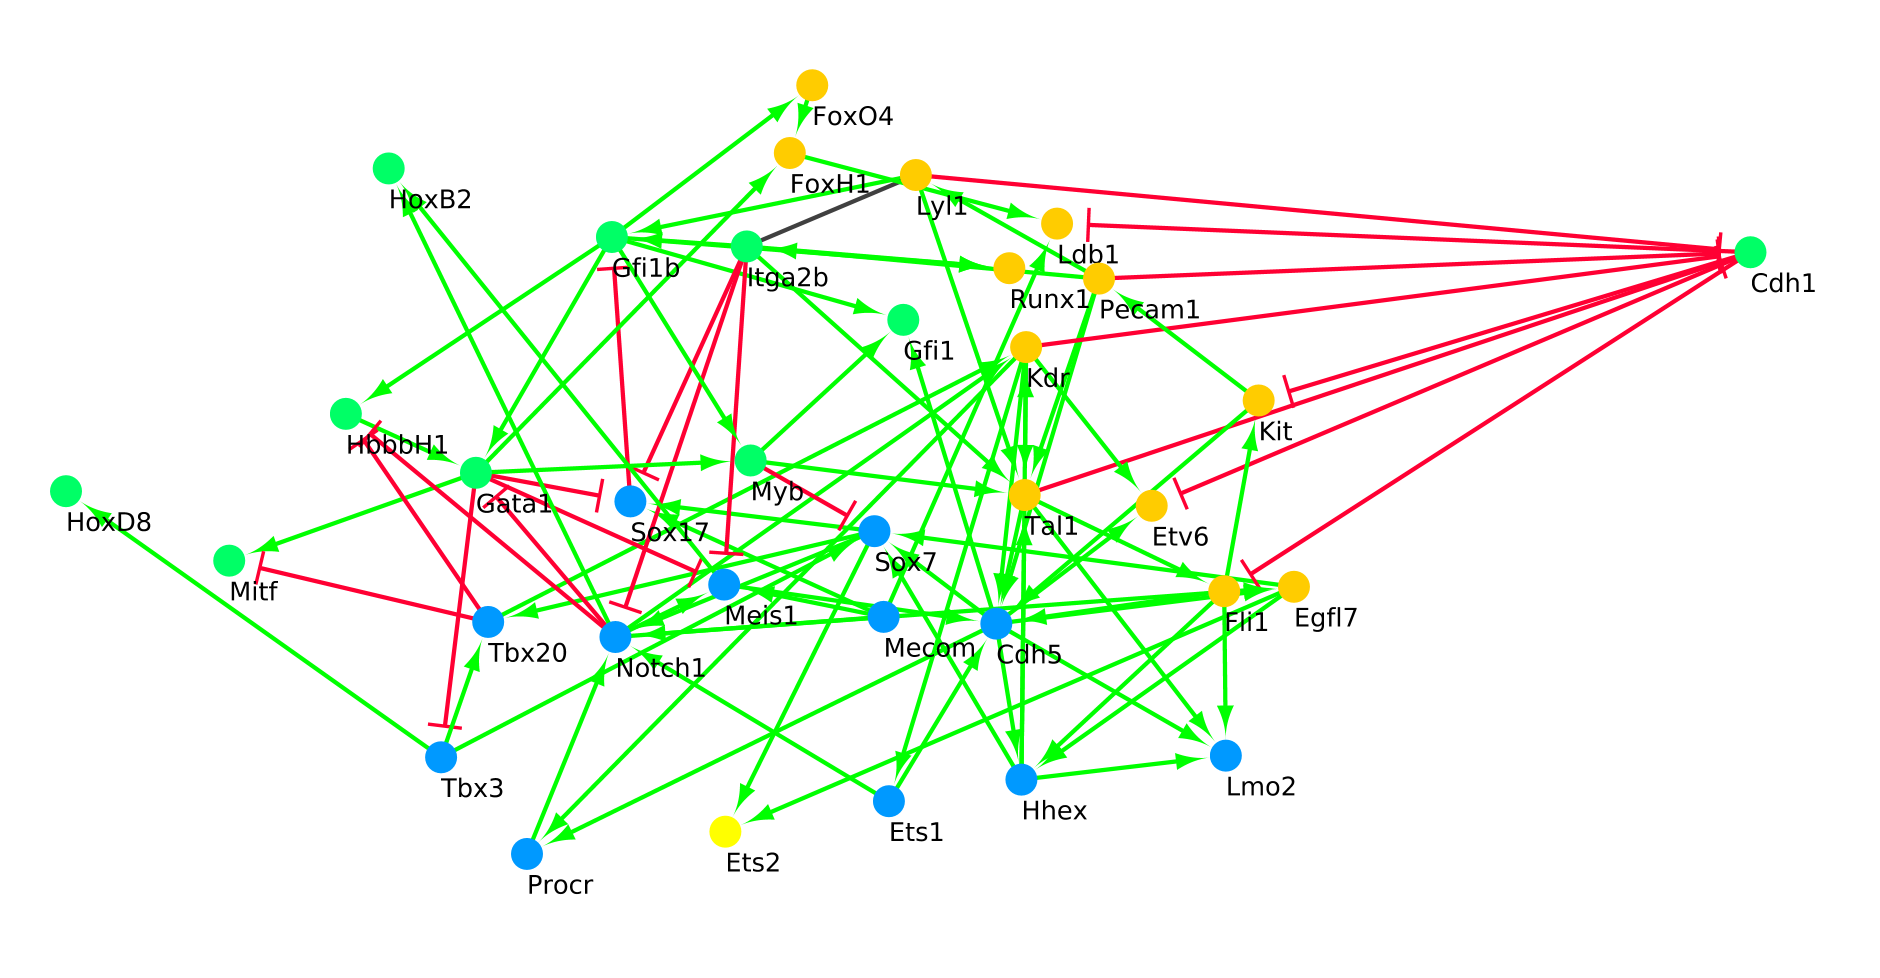
\includegraphics[width =\linewidth]{../Datasets/miic-trimmed/miic-trimmed.png}
		\caption{Network Inferred by MIIC. \textcolor{orange}{Precursor genes}, \textcolor{green}{ Hematopoietic genes} and  \textcolor{blue}{Endothelial genes}}
		\label{fig:miicnetwork}
	\end{figure}

\paragraph{Discussion }The network clearly represents the hematopoietic process as seen by the repression links  infered between the genes classified as hematopoietic and those classified as endothelial. The Cdh1 gene behaves as a regulator ( through repression) of the other precursor genes, if we look back at its gene expression levels we see that the expression drops throughout the differentiation process. This gene was not taken into account in the paper \textit{Learning causal networks with latent variables from multivariate information in genomic data.} (PLoS computational biology 2017, Verny et al.). It leads us to believe that it was wrongly categorized as an hematopoietic gene, that it should rather be categorized as a precursor gene.

\section*{Their Network Inference Method}
The network inference tool used in the article was specially developed for their purpose. And indeed it achieves good results. Moreover it is explanatory, in the sense that it provides the update function of each gene as a boolean fucntion. However, the approach also risks being overly ambitious since the search space is extremely large. We were first tempted to implement it but we finally decided, the amount of work was excessive. Still, we found it interesting to describe their method.

\paragraph{State-transition graph} 
The number of cells is great enough to consider we have all the states the cells can be in. Every pair of states that differ in the expression of exactly one gene are connected to form the state-transition graph.
\paragraph{Network Inference}
Then they search for the direction of the edges as well as the Boolean update function for each of the genes. To do so, they translate their problem into a SAT problem.

\begin{figure}[h!]
	\centering
	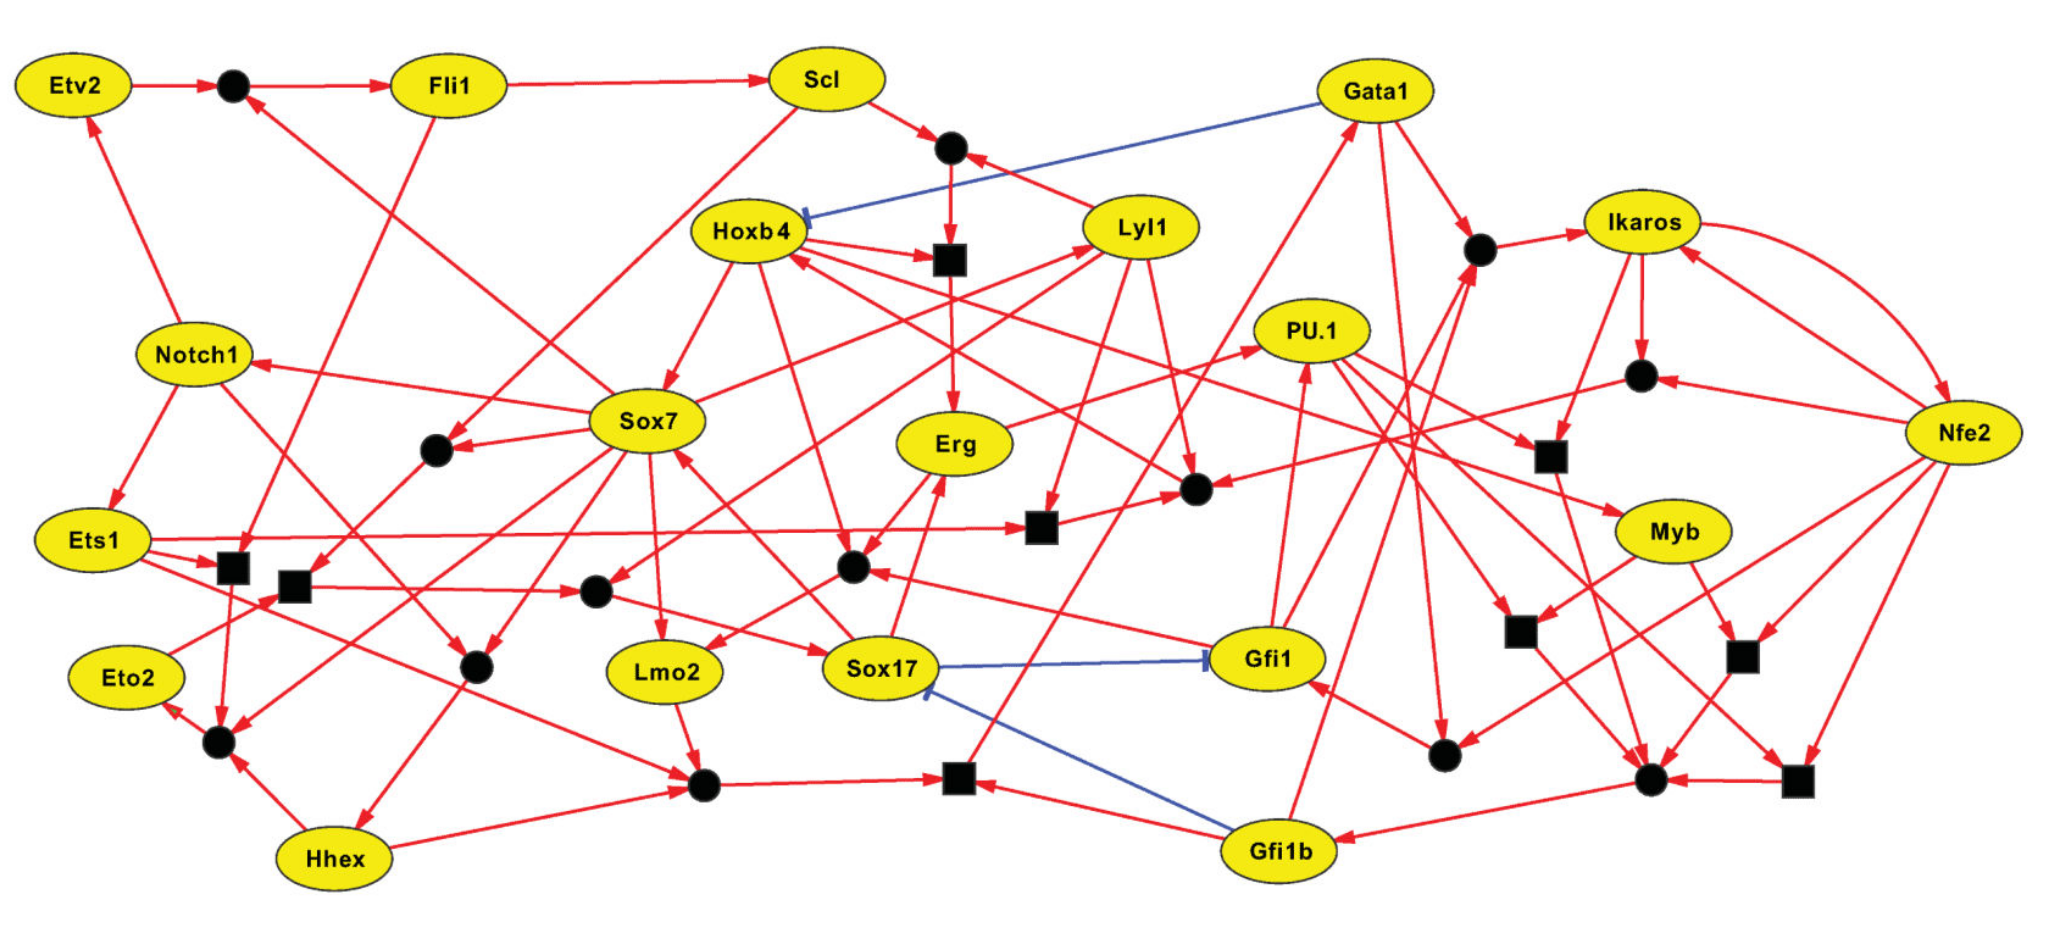
\includegraphics[width = \linewidth]{../Biblio/images/pap_network.png}
	\caption{Network constructed by the SCNS toolkit}
	\label{fig:scns}
\end{figure}

\paragraph{Discussion} One thing interesting about this type of boolean network is that you can find its stable state. A stable state will be assigning a value of expression (ie expressed or not) to each gene such that all boolean equalities are satisfied. We would expect the final cells (those that have already specified) to be stable state of the network. If the 4SG cells are indeed a stable state (or some of them at least) then it does tell that the network is accurate. Also one such network would allow one to simulate the evolution of a cell, it would be interesting to know how well this network fares in doing so.



	
\end{document}